\documentclass[conference]{IEEEtran}
\pdfoutput=1    % For arXiv issues


% -------------------------- COLORBLIND COLORS -------------------------------
% Use color palettes for colorblind people from
% https://davidmathlogic.com/colorblind/#%23D81B60-%231E88E5-%23FFC107-%23004D40 or https://colorbrewer2.org/
\usepackage{xcolor}
\definecolor{wong-black}        {HTML}{000000}
\definecolor{wong-lightorange}  {HTML}{E69F00}
\definecolor{wong-lightblue}    {HTML}{56B4E9}
\definecolor{wong-green}        {HTML}{009E73}
\definecolor{wong-yellow}       {HTML}{F0E442}
\definecolor{wong-darkblue}     {HTML}{0072B2}
\definecolor{wong-darkorange}   {HTML}{D55E00}
\definecolor{wong-pink}         {HTML}{CC79A7}

% -------------------------- PACKAGES -------------------------------

\usepackage{url}
\def\UrlBreaks{\do\/\do-}   % Line breaks of long URLs in biblatex bibliography (https://tex.stackexchange.com/questions/134191/line-breaks-of-long-urls-in-biblatex-bibliography)

\usepackage{hyperref} % Working hyperlink (https://www.overleaf.com/learn/latex/Hyperlinks)
\hypersetup{
    colorlinks=true,
    citecolor=wong-green,
    linkcolor=wong-darkblue,
    filecolor=wong-pink,      
    urlcolor=wong-black,
    pdfpagemode=FullScreen,
    }

% Use these to always use Fig. and Sec. instead of worrying about Figure, Fig, Fig. etc in the document
\newcommand{\figref}[1]{Fig.~\ref{#1}}
\newcommand{\secref}[1]{Sec.~\ref{#1}}

\usepackage{cite}
\usepackage{amsmath,amssymb,amsfonts}
\usepackage{algorithmic}
\usepackage{graphicx}
\usepackage{textcomp}
\usepackage[nolist, nohyperlinks, printonlyused]{acronym} % For consistent acronyms

\def\BibTeX{{\rm B\kern-.05em{\sc i\kern-.025em b}\kern-.08em
    T\kern-.1667em\lower.7ex\hbox{E}\kern-.125emX}}
    
\newcommand\nnfootnote[1]{  % Footnote without hyperref association (https://tex.stackexchange.com/questions/415625/avoiding-hyperref-warning-ignoring-empty-anchor)
  \begin{NoHyper}
  \renewcommand\thefootnote{}\footnote{#1}%
  \addtocounter{footnote}{-1}%
  \end{NoHyper}
}

\begin{document}

% -------------------------- TITLE -------------------------------

\title{A good title is clear, concise and meaningful}

% -------------------------- AUTHORS -------------------------------

\author{\IEEEauthorblockN{Daniel Bogdoll\IEEEauthorrefmark{2}\IEEEauthorrefmark{3}\textsuperscript{\textasteriskcentered},
Author Two\IEEEauthorrefmark{3}\textsuperscript{\textasteriskcentered},
and J. Marius Zöllner\IEEEauthorrefmark{2}\IEEEauthorrefmark{3}}

\IEEEauthorblockA{\IEEEauthorrefmark{2}FZI Research Center for Information Technology, Germany\\
bogdoll@fzi.de}
\IEEEauthorblockA{\IEEEauthorrefmark{3}Karlsruhe Institute of Technology, Germany\\}}

\maketitle

\nnfootnote{\textasteriskcentered~These authors contributed equally}

% -------------------------- ACRONYMS -------------------------------

\begin{acronym}
    \acro{ml}[ML]{Machine Learning}
	\acro{cnn}[CNN]{Convolutional Neural Network}
	\acro{dl}[DL]{Deep Learning}
	\acro{ad}[AD]{Autonomous Driving}
\end{acronym}

% -------------------------- ABSTRACT -------------------------------


\begin{abstract}
Single paragraph up to 250 words. Mini-version of the paper that includes context, state of the art, why it is not good enough, the research question, the methods, the evaluation and conclusions.

\end{abstract}

% -------------------------- KEYWORDS -------------------------------

\begin{IEEEkeywords}
component, formatting, style, styling, insert
\end{IEEEkeywords}

% -------------------------- CONTENT -------------------------------

\section{Introduction}
\label{sec:introduction}

Context of the work. Use \url{https://www.zotero.org/} for your literature management. Every group managed by an FZI employee has unlimited storage for your files. Also, if you want to work offline or in your own IDE, you can simply 'git clone' this project via the menu on the left. Test of all the citations
\cite{Bogdoll_Quantification_2022_arXiv}
\cite{Bogdoll_addatasets_2022_arXiv}
\cite{Bogdoll_Compressing_2021_NeurIPS}
\cite{Bogdoll_Description_2021_ICCV}
\cite{Bogdoll_KIGLIS_2021_ISC2}
\cite{Bogdoll_Taxonomy_2021_arXiv}
\cite{Toettel_Reliving_2021_arXiv}
\cite{Reichert_Towards_2021_ISC2}
\cite{Asam_Openscenario_2020_Web}
\cite{Bogdoll_Augmenting_2017_US}
\cite{Koduri_Aureate_2018_WCX}.

If you refer to figures and sections, please use the commands \textit{figref} and \textit{secref} as shown here: \figref{fig:compare_sensors} and \secref{sec:acknowledgment}. If you want to link to your open-source repository, please use a an href: All code is available on \href{https://github.com/daniel-bogdoll/deep_generative_models}{\color{wong-lightblue}{GitHub}}. \\

Find more details on style here: \url{https://github.com/daniel-bogdoll/ConferenceTemplate/blob/main/README.md}. For inspirations, take a look at awarded papers such as here: \url{https://cvpr2021.thecvf.com/node/329}. If you want to include tables, the \url{https://www.tablesgenerator.com/} is a helpful tool. When you use acronyms, the \textit{acronym} package automatically makes sure that every acronym is spelled out the first time you use it: First time: \ac{ad} and second time: \ac{ad}.

\subsection{Contribution}
Gap statement/research question and contribution. Identify the core contribution. Before you start writing anything it’s important to identify \textbf{the single core contribution} that your paper makes to the field. More text here. Code and data is
available at \href{https://github.com/xxxxx}.


\section{Related Work}
\label{sec:related_work}

\section{Method}
\label{sec:method}

Describe your experimental design with enough detail so that a competent colleague could reproduce your results. Passive voice sometimes functions well in the Methods section.
Elsewhere in a scientific paper, however, it should rarely be chosen. 

\begin{figure}[t]
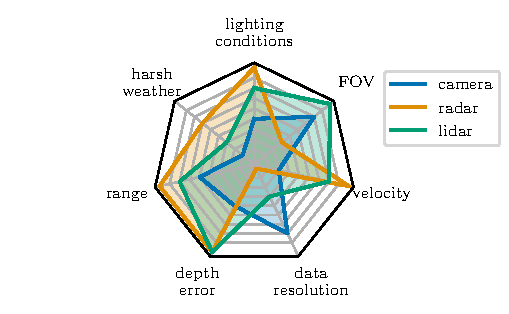
\includegraphics[width=1\columnwidth]{img/spider_sensorcomp.pdf}
\centering
\caption{Figures MUST be in PDF (everything that can be a vector must be a vector) or PNG format to prevent issues with the arXiv upload.}
\label{fig:compare_sensors}
\end{figure}

\section{Evaluation}
\label{sec:evaluation}

%Table from https://www.tablesgenerator.com/
\begin{table}[h!]
\centering
\resizebox{\columnwidth}{!}{%
\begin{tabular}{@{}lllll@{}}
\toprule
Group & Source Domain                   & Target Domain     \\ \midrule
A     & Paintings by Van Gogh           & KITTI             \\
B     & Paintings by Van Gogh           & KITTI + photos    \\
C     & Paintings in Ukiyo-e style      & KITTI             \\
D     & Paintings in Ukiyo-e style      & KITTI + photos    \\
E     & Van Gogh stylized KITTI         & KITTI             \\
F     & Van Gogh stylized Cityscapes    & Cityscapes        
\end{tabular}%
}
\caption{This is an example "booktabs" style table from https://www.tablesgenerator.com/}
\label{table:training}
\end{table}


\section{Conclusion}
\label{sec:conclusion}

Discussion and Outlook
\section{Acknowledgment}
\label{sec:acknowledgment}

This work results partly from the KIGLIS project supported by the German Federal Ministry of Education and Research (BMBF), grant number 16KIS1231.

% -------------------------- REFERENCES -------------------------------

{\small
\bibliographystyle{IEEEtran}
\bibliography{references}
}

\end{document}
